\section{Overall Architecture}
% Code Architecture
Due to the size of the projects code-base and large number of libraries with different \acs{API}s, 
it was necessary to create different object classes with separated concerns,
and a consistent way to use them.

The code base is separated into a backend with code parts that are not visible to the user,
and a front end with each class having an associated \acs{GUI} element.
We also needed main classes to coordinate these responsibilities, handle overall flow,
and serve as a container for anything we did not have time to place in a separate class:
these classes are lib.ts in the backend,
and app.component.ts in the front-end to hold \acs{GUI} elements.

Many of the libraries used have slow, non-blocking IO operations
and make use of callbacks to execute code after the IO operations complete.

Most \acs{GUI} actions result in an event rather than an immediate code execution, 
these events are then caught by app.component
which performs the necessary functionality, through the other classes when relevant.

\begin{table}[H]
	\centering
	\begin{tabular}{l | l}
	    \verb|changing_song|    & User selected a different song to be played \\
		\verb|nextSong|         & User clicked the next song button \\
		\verb|prevSong|         & User clicked the previous song button \\
		\verb|song_ended|       & Song has ended and in line next should be played \\
		\verb|downloaded|       & Song has finished downloading \\
		\verb|ready-for-seed|   & Song is ready to be seeded \\
		\verb|add-song|         & Song added to playlist (from downloads) \\
		\verb|add-song|         & Song added to playlist (from localcontent) \\
		\verb|drop-down-select| & User clicked a search result \\
	\end{tabular}
	\caption{Events used in Streamy}
	\label{table:events}
\end{table}

When the system is started by the browser,
Angular loads the \acs{GUI} elements and then calls ngAfterViewInit in app.component.
ngAfterViewInit performs event bindings, and starts localcontent seeding.
Localcontent retrieves songs stored on the disk, and starts seeding them afterwards using a callback.
All other system functionality is triggered via these events, 
which are driven mostly by user actions and the music player.
\newline

Let us consider some examples: 

The user is searching for a song, and is typing into the search field.

\begin{figure}[H]
	\centerline{
	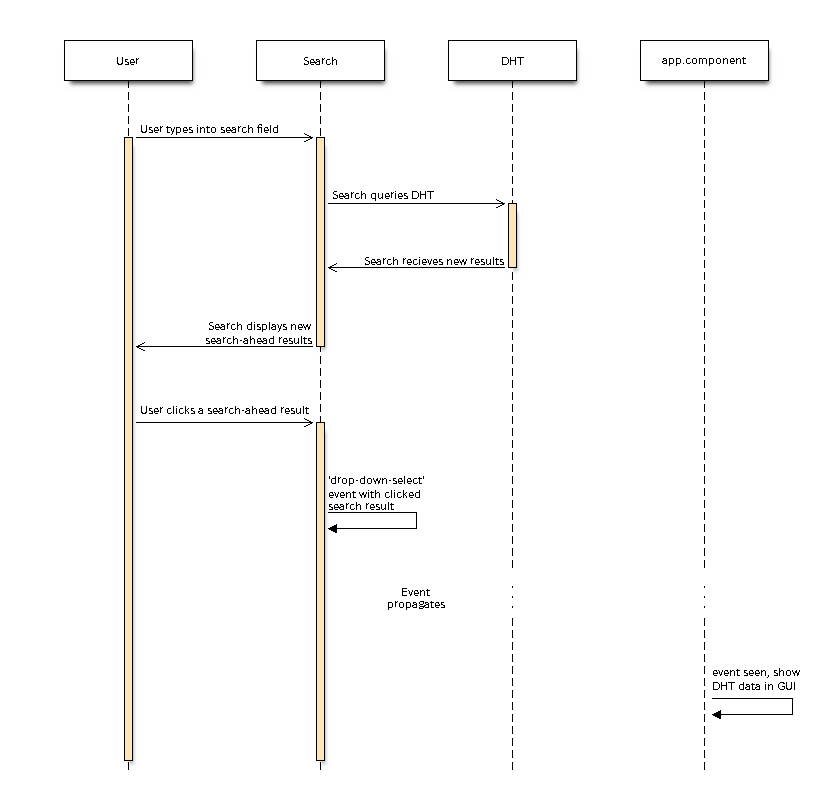
\includegraphics[width=1.5\linewidth]{gfx/searchsong.png}
	}
	\caption{A chart showing the searching process}
	\label{fig:searchsong}
\end{figure}

The event mentioned in \ref{fig:searchsong} will be spread by the Events library,
and is reacted to by eventlisteners in app.component, 
it then updates one of its field variables,
which are then shown to the user via Angular data-binding.

After the user has searched for and found a desired song,
and then clicked the download button.

\begin{figure}[H]
	\centerline{
	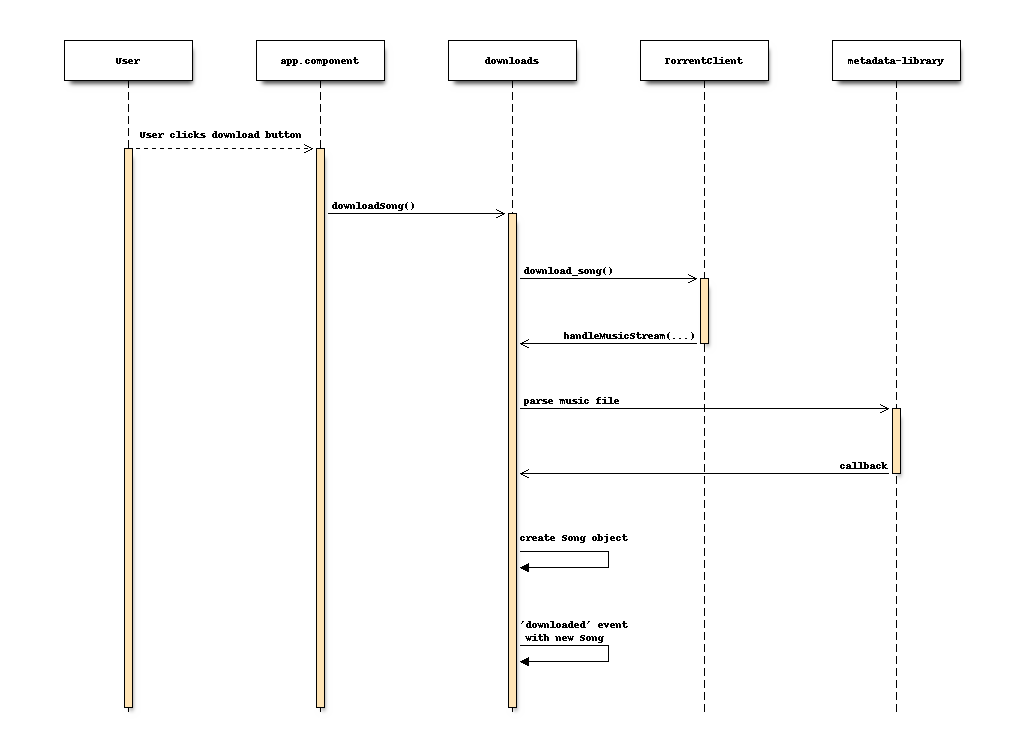
\includegraphics[width=1.5\linewidth]{gfx/downloadsong.png}
	}
	\caption{a chart showing the download process}
	\label{fig:downloadsong}
\end{figure}

The event created in \ref{fig:downloadsong} is then spread by the events library,
and handled in app.component, 
which gives the new song from the event to localcontents addSong() method.
Localcontent adds the new song to its list of seeding content, 
begins seeding it using TorrentClients seed method,
and causes it to appear on the \acs{GUI} using angular databindings.

\begin{figure}[H]
	\centerline{
	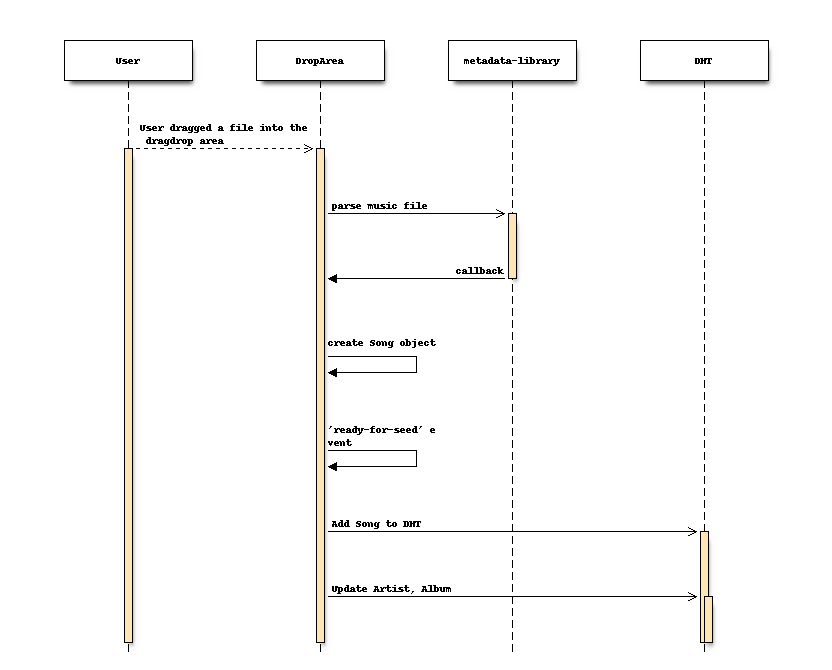
\includegraphics[width=1.5\linewidth]{gfx/dragdrop.png}
	}
	\caption{a chart showing the Drag Drop process}
	\label{fig:dragdrop}
\end{figure}

The DHT update mentioned in \ref{fig:dragdrop} ensures that DHT entries for relevant artists and albums,
contain a reference to this song,
and all the songs it previously referenced.
\newline

% \acs{GUI} (Angular)
The \acs{GUI} needed data-bindings to show torrent information, allow changing songs
and implement a music player \acs{GUI}. 
Angular 2 lets us create \acs{GUI} elements as new \acs{HTML} tags, 
and bootstrap provides generic \acs{GUI} elements and stylesheets for angular, 
they were the easiest way to fill our needs for the \acs{GUI},
so that is what we have used.

Our \acs{GUI} elements consist of a music player interface, a play-list, downloading information 
and show information about local content and seeding.
\newline

\section{How we use Browserify}
% Browserify and why we use it
The project contains a large amount of NodeJS module libraries, 
many of which are designed for NodeJS and not for use in browsers.
We needed some way to use these libraries, and to insure that they are properly loaded.
In NodeJS, modules are loaded and made available by calling the require method 
and assigning the result to a field variable, which can then be used to access the libraries functions.
This capability is not supported natively in browsers, so a tool was needed to provide it.
The Browserify tool takes JavaScript code written for NodeJS, 
transforms it into regular JavaScript code, 
handles all the requires, 
and emits the new JavaScript code as a single easily distributed file called Bundle.js.
Browserify allows our projects end result to consist only of a \acs{HTML} page and one JavaScript file, 
so this seems like an ideal setup, and is what we make use of.
\newline

\section{Song handling}
% How we handle music and music metadata
The program encapsulates the highly inconsistent music files using a Song object,
which contains optional fields corresponding to commonly used meta-data, 
such as title, name of artist, genre and album. 
The Song object also contains information relevant for the BitTorrent system; 
it contains the magnetURI it was retrieved from or is being seeded to, 
it holds the binary file once it is fully available, 
or a reference to the music stream when it is still being downloaded.
This Song object presents all other sections of the project with a uniform way to access meta-data and audio, 
while retaining relational information about which albums or artists the song belongs to. In addition to this, 
we have also created objects to hold information about an album or an artist, 
so we can more easily search for related works in the \acs{DHT}.
\newline

\section{Torrenting}
% WebTorrent
WebTorrent provides seed and download methods using MagnetURI.
Individual downloads and seeds are controlled through a Torrent object provided by WebTorrent,
which contains all the relevant information about progress, 
speed, amount uploaded, number of peers, contained files and so on.
These torrent objects are provided by callbacks at events
and after each called WebTorrent function completes.
The encapsulating torrent.ts class gives access to seed and download methods of WebTorrent, 
but only for our Song Objects, which emphasis the projects intent of being a music streaming service 
rather than generic file sharing application, 
it also provides the WebTorrent torrent object through callbacks to other sections of our code.
\newline

% Granularity of torrents
A torrent is capable of containing one or many files of any format, 
it could contain single music files, whole albums or an artists entire discography.
Our system does not make use of existing torrents made by other applications,
so we are free to choose any granularity best suited for our purposes.
Most music services focus on individual songs, 
as users rarely wish to listen to multiple songs concurrently.
This seems to be the best choice for our project as well, 
but the practicality of what to include in each of our torrents 
could also consider the performance of WebTorrent,
whether it can more efficiently make use of fewer torrents with more included files, 
or if this makes no difference.
\newline

\section{Audio tag limitations}
% Audio Tag and limitations
Modern browsers already support native playback of audio files through the Audio \acs{HTML}5 tag, 
this capability comes with some limitations however.
The audio tag can be provided with a Src property, which defines the file to be played by the browser,
it also comes with a inflexible user interface, provided by the browser.
Ideally, our system would support playback of music files while they are still being downloaded, 
meaning streaming support. 
\acs{HTML}5 Audio only supports only a few music file types,
so we needed some way of combining its functionality with music streaming and an improved user interface.
The render-media library seemed to solve the issue of streaming, it allows the creation of new
audio tags after the browser is loaded, and replacing existing audio tags.
We use render-media to replace the existing audio tag, when the song is changes,
with a new audio tag that contains the new source file, it also seamlessly switches
to use the completed music file when it has completed download.
To fix the Audio tag \acs{GUI}, we have entirely disabled the browser provided interface,
and written our own, making use of Angular 2 and angular-Bootstrap 2.
\newline

% LocalStorage vs LocalForage
\section{Fixing Browser Storage}
To have persistency in user sessions, we needed a way of storing data to the disk. There are several standard ways to store data in web browsers, but all of these have their own drawbacks.

Traditional browser cookies can store up to 4KB of data, 
not enough to save even one song. 
To store a song in cookies we would need to create thousands of cookies, 
and store small parts of a song in each one, 
this seemed like a difficult and inelegant solution.

Seeing the need for larger storage spaces, 
industry concerns have added LocalStorage to the \acs{HTML} 5 standard,
which allows websites to store arbitrarily large amounts of data,
but this again suffers significant drawbacks: 
implementation varies greatly between browsers, 
and can in some cases be wiped after reaching only 5 megabytes, 
hardly enough for our purposes.

Some browsers have also added support for database storage, via IndexedDB and WebSQL \citep{WebSQL}, 
but this is not supported in every browser. 
For the sake of not excluding any browser that might work with WebTorrent, but not with IndexedDB,
it seemed like we needed a better solution.
\newline

To overcome these challenges, we use a library called localForage, 
which checks what the host browser supports,
and makes use of the best available storage method.
We found through experiments
that localForage has issues storing JavaScript objects to disk when these objects contain large binary blobs, 
these could consume as much as 4 gigabytes of space for an originally 5MB music file.
Separating the generated meta-data object and song binary before placing the in storage
seemed to solve this issue.
\newline

% Storage
The object-blob separation behavior and use of localforage,
needed to be consistent throughout the project, 
so we created a Storage class which uses localforage and handles the data separation implicitly when its storage methods are called.
We have also disallowed the direct use of localforage anywhere else:
all other sections of the project should save and get data through using the Storage class to ensure consistent behavior. 
This was done by removing any inclusion of the localforage library outside of the Storage class file.

As local content should also be visible in the \acs{GUI}, 
be seeded and be capable of being added to the playing,
we created another class called LocalContent,
which retrieves all songs from the disk at start-up,
begins to seed them, making them available for other users in the network to download,
and presents a \acs{GUI} element to the user.
\newline

\section{Tracker Implementation}
In our implementation, we've disregarded the manual peer input model, as it is
not user friendly. As such we're left with tracker-based and trackerless, as 
we've limited ourselves to the context of the browser, we're bound to using 
WebRTC, and by extension we need a centralized component to bootstrap these
connections. 

We are however, in theory, free to pick whether we want to use a tracker, or 
utilize a trackerless \acs{DHT} for bootstrapping peers, but only in theory as our
WebRTC-based BitTorrent implementation (as previously mentioned here) does
indeed not support trackerless, and as the provided WebSocket tracker for 
WebTorrent fulfills both the role of bootstrapping WebRTC connections, and the
role of the BitTorrent tracker.

As previously mentioned, had we been able to utilize trackerless, we've been
able to use the trackerless \acs{DHT} as our searching \acs{DHT}, however utilizing a
tracker provides other unique capabilities, namely; centralized control of the
swarm. 
\newline
- A content distributor might like to have this capability, to do data
processing on popular content, or otherwise track the swarm.

While a tracker-based solution utilizes a centralized components, it is not
limited to just using one. Our solution utilizes the 4 default trackers
provided by WebTorrent, but it's trivial to run your own tracker and add it to
the resources in the network.
\newline
- A content provider may want to track how often it's content is downloaded,
and could add the content to the network with just one tracker being their own.
